\documentclass{article}
\usepackage{stackengine}
%\usepackage[utf8]{inputenc}
\usepackage[T1]{fontenc}
\usepackage{amsmath}
\usepackage{amsfonts}
\usepackage{graphicx}
\usepackage{pbsi}
\usepackage{lmodern}
\usepackage[a5paper]{geometry}
\usepackage{pdflscape}
\usepackage[dvipsnames, svgnames]{xcolor}
\usepackage[pages=some]{background}
\usepackage{tikz}
\usetikzlibrary{math} 
\usetikzlibrary{automata,positioning}
\usetikzlibrary[decorations.text]

%\usetikzlibrary[automata]

\usetikzlibrary{calc}
\newcommand*{\vertchar}[2][0pt]{%
  \tikz[
    inner sep=1pt,
    shorten >=-.15ex,
    shorten <=-.15ex,
    line cap=round,
    baseline=(c.base),
  ]\draw
    (0,0) node (c) {#2}
    ($(c.north)+(#1,0)$) -- ($(c.north)+(#1,0)$);%
}


\makeatletter
\newcommand{\dotr}[1]{%
  \mathpalette\@dotr{#1}%
}

\newcommand*{\@dotr}[2]{%
  % #1: math style (\displaystyle, ..., \scriptscriptstyle)
  % #2: argument of \dotr
  \sbox0{$\m@th#1#2$}%
  \usebox{0}%
  % simulating a superscript
  %\raisebox{\dimexpr\ht0-\height}{$\m@th#1\addvbuffer[-1ex 0.9ex]{.}}%
  \raisebox{3.5pt}{$\m@th#1\@smallbullet#1\bullet$}%
  \kern\scriptspace
}
\newcommand*{\@smallbullet}[2]{%
  \scalebox{.3}{$\m@th#1#2$}%
}
\makeatother
    
\newcommand*{\siin}[1]{\stackinset{c}{}{b}{5.5pt}{\small\ttfamily\char'15}{#1}}
\newcommand*{\nn}{\textsuperscript{n}}

\newcommand*{\pehin}[1]{\stackinset{c}{}{b}{5.5pt}{\small\ttfamily\char'15}{#1}}
\newcommand*{\dtr}{\raisebox{3.5pt}{$\scalebox{.3}{$\bullet$}$}}
\newcommand*{\dtrh}{\raisebox{5pt}{$\scalebox{.3}{$\bullet$}$}}



\begin{document}

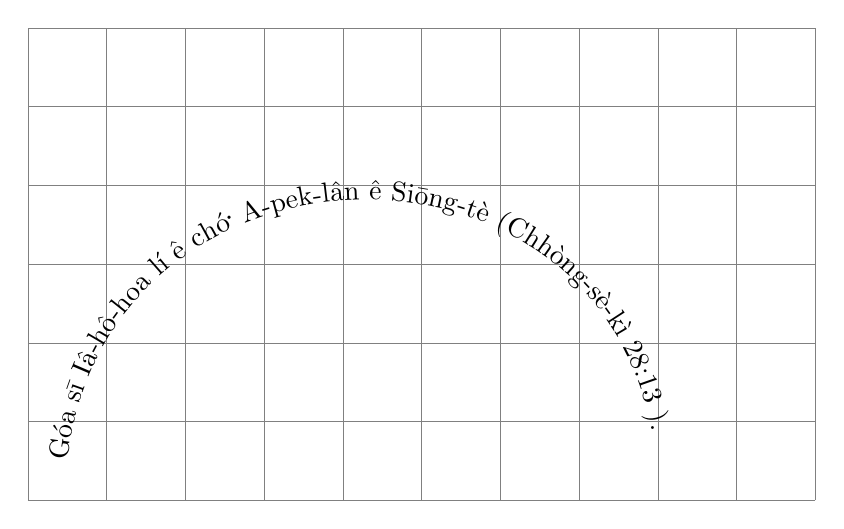
\begin{tikzpicture} 
\draw [help lines] grid (10,6); 
\path [
postaction={decoration={text along path, 
text={G{\'{o}}a s{\={\i}} I{\^{a}}-h{\^{o}}-hoa l{\'{\i}} {\^{e}} ch{\'{o}}{\dtr} A-pek-l{\^{a}}n {\^{e}} Si{\={o}}ng-t{\`{e}}  (Chh{\`{o}}ng-s{\`{e}}-k{\`{\i}} 28:13 ). }, 
text align={align=left}}, decorate}
] (0.5,0.5) .. controls (1, 5) and (8,5) .. (8,0); 
\end{tikzpicture}


\vspace*{1cm}
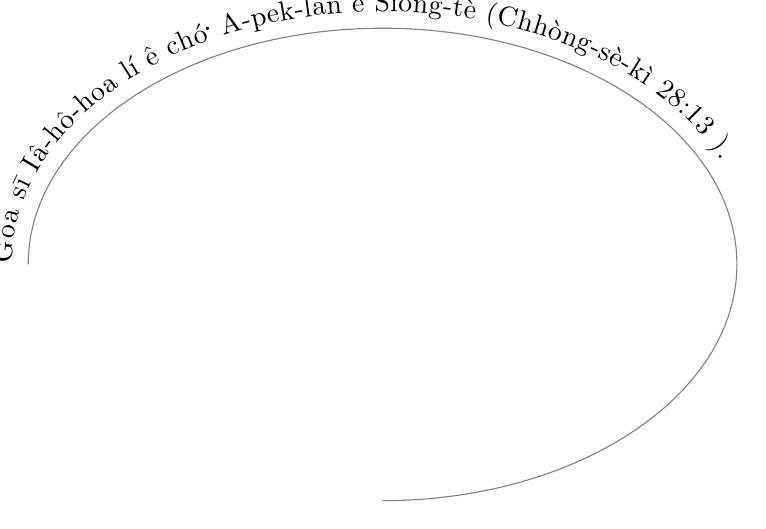
\begin{tikzpicture} 
%\draw [help lines] grid (3,2); 
\fill [
draw=gray,fill=white!20, 
postaction={decorate,decoration={
raise=6pt,text along path, text={ G{\'{o}}a s{\={\i}} I{\^{a}}-h{\^{o}}-hoa l{\'{\i}} {\^{e}} ch{\'{o}}{\dtr} A-pek-l{\^{a}}n {\^{e}} Si{\={o}}ng-t{\`{e}}  (Chh{\`{o}}ng-s{\`{e}}-k{\`{\i}} 28:13 ). }
}}
] (0,1) arc (180:-90:4.5cm and 3cm); 
\end{tikzpicture}

\vspace*{-20mm}
\hspace*{2mm}
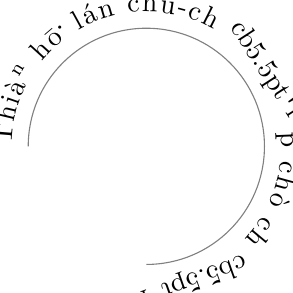
\begin{tikzpicture} 
%\draw [help lines] grid (3,2); 
\fill [
draw=gray,fill=white!20, 
postaction={decorate,decoration={
raise=6pt,text along path, text={  Thi{\`{a}}{\nn} h{\={o}}{\dtr} l{\'{a}}n ch{\={u}}-ch{\pehin{\i}}p ch{\`{o}} ch{\pehin{\i}}t-h{\'{o}}e}
}}
] (0,1) arc (180:-90:1.5cm and 1.5cm); 
\end{tikzpicture}



\end{document}